\part{Khám phá dữ liệu nguồn (EDA)}
\label{part:ch2}

Trước khi thiết kế đường ống xử lý trên bộ nhớ và các thuật toán dự báo, nhóm thực hiện kiểm toán toàn diện hai tập dữ liệu thô bằng kịch bản phân tích tự động \mintinline{text}{scripts/eda_report.js}. Chương này trình bày các phát hiện thực nghiệm từ bộ dữ liệu bán lẻ giày dép và trang phục. Mục~\ref{sec:ch2-script} mô tả quy trình trích xuất EDA tái lập. Mục~\ref{sec:ch2-audit} trình bày kết quả kiểm toán giá trị thiếu, quy ước hoàn trả âm và các bất thường dữ liệu. Mục~\ref{sec:ch2-sales-eda} phân tích xu hướng mùa vụ theo tháng, cơ cấu nhóm hàng, top $10$ danh mục và độ phân tán giữa $40$ cửa hàng, còn Mục~\ref{sec:ch2-inv-eda} đánh giá phân bố trạng thái giá và sức khỏe tồn kho trên toàn bộ $284.755$ bản ghi.

\section{Quy trình khám phá dữ liệu tái lập}
\label{sec:ch2-script}

\begin{figure}[H]
	\centering
	\mermaidfile[width=0.95\linewidth, keepaspectratio]{diagrams/eda_pipeline.mmd}
	\caption{Quy trình trích xuất và kiểm toán EDA tự động trong \texttt{scripts/eda\_report.js}}
	\label{fig:eda_pipeline}
\end{figure}

Trong mã nguồn ban đầu, các thống kê khám phá dữ liệu chỉ được tính cục bộ cho $4$ biểu đồ trên thẻ \textbf{EDA \& Streaming}. Để kiểm chứng giả thuyết mùa vụ, kiểm tra chất lượng từng cột và đánh giá phân bố toàn bộ $284.755$ bản ghi tồn kho, nhóm bổ sung kịch bản \mintinline{text}{scripts/eda_report.js} (Hình~\ref{fig:eda_pipeline}). Kịch bản đọc luồng hai tập tin CSV thông qua \mintinline{text}{csv-parser}, tái sử dụng hàm \mintinline{javascript}{classifyInventory} từ tầng thuật toán lõi và xuất kết quả chuẩn hóa sang \mintinline{javascript}{data/results/eda_summary.json} trong $3.305\text{ ms}$.

\medskip

Mã nguồn~\ref{lst:eda-stats} minh họa hàm \mintinline{text}{computeNumericStats} dùng để tính các phân vị (\textit{median}, $P_{95}$) và giá trị cực trị trên toàn bộ tập dữ liệu mà không làm biến đổi mảng gốc.

\begin{listing}[H]
	\begin{minted}[fontsize=\footnotesize, linenos, breaklines, firstnumber=26]{javascript}
function computeNumericStats(values) {
  if (!values || values.length === 0) {
    return { count: 0, sum: 0, min: 0, median: 0, p95: 0, max: 0, mean: 0 };
  }
  const sorted = [...values].sort((a, b) => a - b);
  const n = sorted.length;
  let sum = 0;
  for (let i = 0; i < n; i++) sum += sorted[i];
  const mid = Math.floor(n / 2);
  const median = n % 2 === 0 ? (sorted[mid - 1] + sorted[mid]) / 2 : sorted[mid];
  const p95Idx = Math.min(n - 1, Math.floor(0.95 * (n - 1)));
  return {
    count: n, sum: roundTo(sum, 2), min: roundTo(sorted[0], 4),
    median: roundTo(median, 4), p95: roundTo(sorted[p95Idx], 4),
    max: roundTo(sorted[n - 1], 4), mean: roundTo(sum / n, 4)
  };
}
\end{minted}
	\caption{Hàm tính thống kê mô tả và phân vị trong \texttt{scripts/eda\_report.js}}
	\label{lst:eda-stats}
\end{listing}

\section{Kiểm toán chất lượng và Thống kê mô tả}
\label{sec:ch2-audit}
Kết quả rà soát từng cột trên $125.751$ bản ghi bán hàng và $284.755$ bản ghi tồn kho chỉ ra bốn đặc điểm chất lượng dữ liệu quan trọng:
\begin{itemize}[topsep=0pt, itemsep=1pt]
	\item \textbf{Khuyết hoàn toàn lý do hoàn trả:} $16/17$ cột của tập bán hàng và $18/18$ cột của tập tồn kho có tỷ lệ thiếu bằng $0\%$. Riêng cột \mintinline{text}{Reason of Return} trống ở toàn bộ $125.751$ dòng ($100\%$), kể cả trên $7.491$ giao dịch có \mintinline{text}{Is Return = 1}. Vì vậy, phân tích hoàn trả chỉ dựa trên cờ nhị phân \mintinline{text}{Is Return}.
	\item \textbf{Mã hóa hoàn trả bằng giá trị âm:} Toàn bộ $7.491$ giao dịch có \mintinline{text}{Is Return = 1} đều ghi nhận đồng thời \mintinline{text}{Qty Sold < 0} và \mintinline{text}{Sales Amount < 0} (cùng \mintinline{text}{Cogs < 0}). Nhờ vậy, phép cộng dồn doanh thu và sản lượng theo tháng tự động phản ánh doanh số thuần sau hoàn trả.
	\item \textbf{Giá trị âm và mốc giả trong tập tồn kho:} Cột \mintinline{text}{Qty on hand} xuất hiện giá trị âm (nhỏ nhất $-9$, phản ánh lệch kiểm kê hoặc giữ chỗ vượt tồn), đồng thời $22.701$ bản ghi ($7{,}97\%$) mang mốc kết thúc giả \mintinline{text}{End Date = 9999-12-31} đại diện cho trạng thái đang còn hiệu lực.
	\item \textbf{Tập trung đơn vị nhỏ và lệch phải:} Trung vị (\textit{median}) của \mintinline{text}{Qty Sold} bằng $1$ (bách phân vị $P_{95} = 1$, cực đại $14$) và trung vị \mintinline{text}{Qty on hand} bằng $2$ ($P_{95} = 6$, cực đại $56$), cho thấy đặc trưng bán lẻ từng đôi/chiếc với một số ít đơn hàng sỉ hoặc lô lớn.
\end{itemize}

\begin{table}[H]
	\centering
	\footnotesize
	\setlength{\tabcolsep}{4pt}
	\begin{tabular}{p{4.1cm} l r r r r r r}
		\toprule
		\textbf{Trường dữ liệu}                     & \textbf{Tập tin} & \textbf{Tổng cộng} & \textbf{Min} & \textbf{Median} & \textbf{$P_{95}$} & \textbf{Max} & \textbf{Trung bình} \\
		\midrule
		\mintinline{text}{Qty Sold}                 & Sales            & $116.995$          & $-3$         & $1$             & $1$               & $14$         & $0{,}93$            \\
		\mintinline{text}{Sales Amount}             & Sales            & $10.482.110{,}25$  & $-380{,}00$  & $90{,}00$       & $165{,}00$        & $2.660{,}00$ & $83{,}36$           \\
		\mintinline{text}{Cogs}                     & Sales            & $5.847.751{,}10$   & $-192{,}28$  & $50{,}05$       & $86{,}02$         & $1.345{,}96$ & $46{,}50$           \\
		\mintinline{text}{Qty on hand}              & Inventory        & $653.407$          & $-9$         & $2$             & $6$               & $56$         & $2{,}29$            \\
		\mintinline{text}{Stock Unit Selling Price} & Inventory        & $27.140.901{,}90$  & $0{,}00$     & $100{,}00$      & $165{,}00$        & $250{,}00$   & $95{,}31$           \\
		\mintinline{text}{Stock Unit Cost Price}    & Inventory        & $13.502.936{,}28$  & $-16{,}94$   & $50{,}05$       & $82{,}60$         & $336{,}38$   & $47{,}42$           \\
		\bottomrule
	\end{tabular}
	\caption{Thống kê mô tả các biến định lượng trong bộ dữ liệu}
	\label{tab:eda-numeric-stats}
\end{table}

\section{Phân tích Hành vi bán hàng và Tính mùa vụ}
\label{sec:ch2-sales-eda}
Tập tin \mintinline{text}{retail_sales_ml_apl.csv} trải dài $11$ tháng từ \texttt{2025-06-01} đến \texttt{2026-04-24}, bao phủ $2.326$ mã sản phẩm, $27$ danh mục và $40$ cửa hàng trên một kênh duy nhất (\textit{Channel Alpha}). Bảng~\ref{tab:eda-monthly} và Hình~\ref{fig:eda-monthly-chart} cho thấy hai đỉnh mùa vụ rõ rệt: tháng \textbf{2025-08} ($1{,}535$ triệu USD, mùa tựu trường) và tháng \textbf{2025-12} ($1{,}786$ triệu USD, mùa lễ hội cuối năm), cao gấp $2{,}0$--$3{,}1$ lần các tháng thấp điểm như \textbf{2026-01} ($565{,}3$ nghìn USD) hay \textbf{2026-04} ($507{,}1$ nghìn USD, chỉ ghi nhận đến ngày $24/04$). Đáng chú ý, tỷ lệ hoàn trả tăng vọt lên \textbf{$9{,}81\%$} vào tháng \textbf{2026-01} ngay sau đợt mua sắm tháng $12$, kéo biên lợi nhuận gộp xuống thấp nhất chuỗi ($40{,}45\%$). Chính biến động mạnh theo chu kỳ tháng này là cơ sở thực nghiệm để thuật toán \textit{Super Forecast} bổ sung hệ số mùa vụ thay cho trung bình trượt đơn giản.

\begin{figure}[H]
	\centering
	\footnotesize
	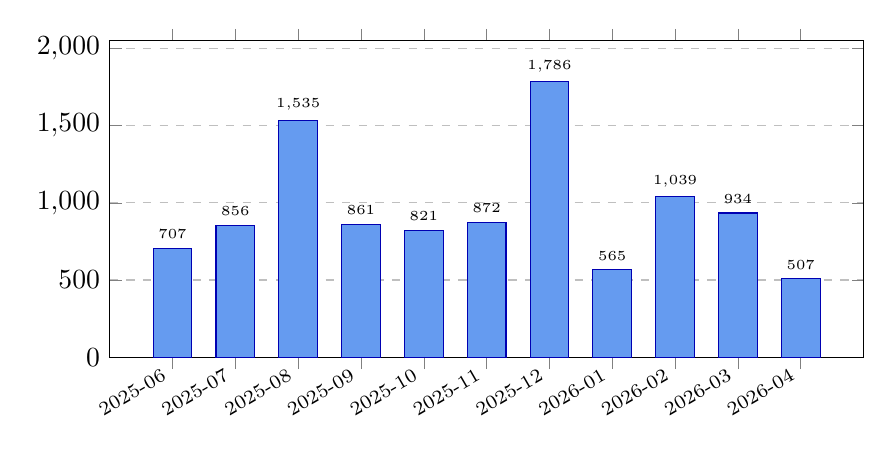
\begin{tikzpicture}
		\begin{axis}[
				width=0.92\linewidth,
				height=5.6cm,
				ybar,
				bar width=14pt,
				ymin=0,
				ymax=2050,
				symbolic x coords={2025-06,2025-07,2025-08,2025-09,2025-10,2025-11,2025-12,2026-01,2026-02,2026-03,2026-04},
				xtick=data,
				x tick label style={rotate=30, anchor=east, font=\scriptsize},
				ymajorgrids=true,
				grid style=dashed,
				nodes near coords,
				nodes near coords style={font=\tiny, rotate=0, anchor=south},
				every node near coord/.append style={/pgf/number format/fixed, /pgf/number format/precision=0},
			]
			\addplot[fill=SkyBlue!75!blue, draw=blue!70!black] coordinates {
					(2025-06, 706.7)
					(2025-07, 855.6)
					(2025-08, 1535.1)
					(2025-09, 860.5)
					(2025-10, 821.3)
					(2025-11, 871.9)
					(2025-12, 1785.5)
					(2026-01, 565.3)
					(2026-02, 1039.0)
					(2026-03, 934.2)
					(2026-04, 507.1)
				};
		\end{axis}
	\end{tikzpicture}
	\caption{Xu hướng doanh thu theo tháng từ dữ liệu thực nghiệm (nghìn USD)}
	\label{fig:eda-monthly-chart}
\end{figure}

\begin{table}[H]
	\centering
	\footnotesize
	\setlength{\tabcolsep}{4.5pt}
	\begin{tabular}{c r r r r r r}
		\toprule
		\textbf{Tháng}   & \textbf{Số giao dịch} & \textbf{Hoàn trả} & \textbf{Tỷ lệ hoàn (\%)} & \textbf{Qty Sold} & \textbf{Doanh thu (\$)} & \textbf{Biên gộp (\%)} \\
		\midrule
		\texttt{2025-06} & $8.328$               & $464$             & $5{,}57$                 & $7.712$           & $706.683{,}44$          & $47{,}12$              \\
		\texttt{2025-07} & $10.120$              & $547$             & $5{,}41$                 & $9.545$           & $855.571{,}55$          & $45{,}91$              \\
		\texttt{2025-08} & $18.517$              & $829$             & $4{,}48$                 & $17.561$          & $1.535.117{,}21$        & $45{,}83$              \\
		\texttt{2025-09} & $10.499$              & $663$             & $6{,}31$                 & $9.654$           & $860.457{,}23$          & $43{,}30$              \\
		\texttt{2025-10} & $9.750$               & $543$             & $5{,}57$                 & $9.226$           & $821.266{,}08$          & $42{,}82$              \\
		\texttt{2025-11} & $10.118$              & $545$             & $5{,}39$                 & $9.527$           & $871.946{,}34$          & $44{,}53$              \\
		\texttt{2025-12} & $19.798$              & $1.381$           & $6{,}98$                 & $18.717$          & $1.785.534{,}95$        & $44{,}60$              \\
		\texttt{2026-01} & $7.955$               & $780$             & $9{,}81$                 & $6.609$           & $565.272{,}83$          & $40{,}45$              \\
		\texttt{2026-02} & $10.944$              & $671$             & $6{,}13$                 & $10.222$          & $1.038.967{,}86$        & $45{,}84$              \\
		\texttt{2026-03} & $12.902$              & $701$             & $5{,}43$                 & $11.882$          & $934.194{,}48$          & $40{,}50$              \\
		\texttt{2026-04} & $6.820$               & $367$             & $5{,}38$                 & $6.340$           & $507.098{,}28$          & $41{,}96$              \\
		\bottomrule
	\end{tabular}
	\caption{Diễn biến doanh thu, sản lượng và tỷ lệ hoàn trả qua 11 tháng}
	\label{tab:eda-monthly}
\end{table}

Xét theo cơ cấu sản phẩm, giá bán và cửa hàng:
\begin{itemize}[topsep=0pt, itemsep=1pt]
	\item \textbf{Nhóm sản phẩm (\textit{Product Division}):} \textit{Scholar Footwear} dẫn đầu với $76.907$ giao dịch ($7{,}338$ triệu USD, tỷ lệ hoàn trả $5{,}93\%$); \textit{Femme Footwear} đạt $29.848$ giao dịch ($2{,}712$ triệu USD) nhưng có tỷ lệ hoàn trả cao nhất ($7{,}74\%$); \textit{Junior Apparel} đạt $18.996$ giao dịch ($431{,}7$ nghìn USD) với tỷ lệ hoàn trả thấp nhất ($3{,}28\%$).
	\item \textbf{Loại hình bán hàng (\textit{Sales Type}):} Bán nguyên giá (\textit{Full Price}) chiếm $74{,}69\%$ ($93.929$ dòng), tiếp theo là \textit{Promo} ($18{,}81\%$), \textit{Markdown Tier 1} ($3{,}49\%$), \textit{Markdown Tier 2} ($1{,}94\%$) và \textit{Clearance} ($1{,}08\%$).
	\item \textbf{Độ phân tán giữa $40$ cửa hàng:} Doanh thu trung bình mỗi cửa hàng đạt $262.052{,}76$ USD (trung vị $263.160{,}82$ USD), nhưng chênh lệch giữa cửa hàng dẫn đầu (\texttt{STR-1006}: $485.561{,}44$ USD) và cửa hàng thấp nhất (\texttt{STR-1344}: $139.220{,}10$ USD) lên tới $3{,}49$ lần. Điều này chứng minh việc dự báo nhu cầu cần tách theo từng cặp \textit{Danh mục -- Cửa hàng} thay vì gộp chung toàn chuỗi.
\end{itemize}
Bảng~\ref{tab:eda-top10} liệt kê $10$ danh mục bán chạy nhất theo \mintinline{text}{Qty Sold}, chiếm $95.605 / 116.995$ đơn vị ($81{,}72\%$ tổng sản lượng toàn chuỗi).
\begin{table}[H]
	\centering
	\footnotesize
	\begin{tabular}{c p{6cm} r r}
		\toprule
		\textbf{Hạng} & \textbf{Product Category}                           & \textbf{Qty Sold} & \textbf{Doanh thu (\$)} \\
		\midrule
		$1$           & \mintinline{text}{Scholar Footwear Trailblazer}     & $20.584$          & $1.909.759{,}99$        \\
		$2$           & \mintinline{text}{Scholar Footwear Retro Legend}    & $12.569$          & $1.920.958{,}56$        \\
		$3$           & \mintinline{text}{Femme Footwear Trailblazer}       & $12.325$          & $1.238.790{,}65$        \\
		$4$           & \mintinline{text}{Scholar Footwear Modern Legend}   & $10.731$          & $1.062.646{,}92$        \\
		$5$           & \mintinline{text}{Scholar Footwear Court Casual}    & $9.530$           & $702.385{,}90$          \\
		$6$           & \mintinline{text}{Scholar Footwear Flight Classic}  & $8.926$           & $767.298{,}33$          \\
		$7$           & \mintinline{text}{Femme Footwear Court Casual}      & $7.279$           & $647.820{,}37$          \\
		$8$           & \mintinline{text}{Scholar Footwear Boot Collection} & $6.049$           & $660.152{,}85$          \\
		$9$           & \mintinline{text}{Junior Apparel Crew Tees}         & $4.078$           & $86.652{,}57$           \\
		$10$          & \mintinline{text}{Junior Apparel Printed Tees}      & $3.534$           & $39.928{,}08$           \\
		\bottomrule
	\end{tabular}
	\caption{Top 10 danh mục sản phẩm có sản lượng bán cao nhất}
	\label{tab:eda-top10}
\end{table}

\section{Phân tích Tồn kho và Phân bố sức khỏe toàn cục}
\label{sec:ch2-inv-eda}
Trên $284.755$ bản ghi của \mintinline{text}{retail_inventory_ml_apl.csv}, trạng thái giá \textit{Full Price} chiếm tỷ trọng áp đảo $91{,}97\%$ ($261.899$ dòng), theo sau là \textit{Markdown Tier 1} ($4{,}25\%$), \textit{Markdown Tier 2} ($2{,}44\%$), \textit{Clearance} ($1{,}33\%$) và \textit{Promo} ($0{,}01\%$). Tổng giá trị bán lẻ hàng tồn đạt $63{,}90$ triệu USD trên tổng giá vốn $31{,}62$ triệu USD.

\medskip

Khi áp dụng hàm phân loại \mintinline{javascript}{classifyInventory} (sử dụng cửa sổ $30$ ngày cuối từ \texttt{2026-03-25} đến \texttt{2026-04-24}, gồm $9.244$ giao dịch) lên toàn bộ $284.755$ bản ghi tồn kho, kết quả phân bố toàn cục như sau (Bảng~\ref{tab:eda-inv-health}):
\begin{itemize}[topsep=0pt, itemsep=1pt]
	\item \textbf{Healthy ($49{,}33\%$):} Gồm $140.479$ bản ghi, nhưng có tới $73.247$ bản ghi ($25{,}72\%$ toàn kho) rơi vào nhánh dự phòng $\text{avgDailySales} \le 0$ (không có doanh số trong $30$ ngày gần nhất). Chỉ $67.232$ bản ghi ($23{,}61\%$) thực sự nằm trong vùng an toàn $14 \le \text{Cover} < 60$ ngày.
	\item \textbf{Low Stock ($43{,}98\%$):} $125.240$ bản ghi có độ bao phủ dưới $14$ ngày bán, cho thấy rủi ro đứt hàng phổ biến trên các mã có sức mua cao gần đây.
	\item \textbf{Overstock ($6{,}69\%$):} $19.036$ bản ghi có tồn kho vượt ngưỡng $60$ ngày bán, tập trung vốn lưu động cần đẩy mạnh giảm giá.
\end{itemize}

\begin{table}[H]
	\centering
	\footnotesize
	\setlength{\tabcolsep}{4pt}
	\begin{tabular}{p{3.6cm} r r | p{4.6cm} r r}
		\toprule
		\textbf{Stock Status (CSV)}        & \textbf{Số dòng} & \textbf{Tỷ lệ (\%)} & \textbf{Phân loại thuật toán}     & \textbf{Số dòng} & \textbf{Tỷ lệ (\%)} \\
		\midrule
		\mintinline{text}{Full Price}      & $261.899$        & $91{,}97$           & \textbf{Healthy} (Tổng)           & $140.479$        & $49{,}33$           \\
		\mintinline{text}{Markdown Tier 1} & $12.091$         & $4{,}25$            & \quad \textit{Trong vùng 14--60d} & $67.232$         & $23{,}61$           \\
		\mintinline{text}{Markdown Tier 2} & $6.937$          & $2{,}44$            & \quad \textit{Nhánh bán $\le 0$}  & $73.247$         & $25{,}72$           \\
		\mintinline{text}{Clearance}       & $3.798$          & $1{,}33$            & \textbf{Low Stock} ($< 14$d)      & $125.240$        & $43{,}98$           \\
		\mintinline{text}{Promo}           & $30$             & $0{,}01$            & \textbf{Overstock} ($\ge 60$d)    & $19.036$         & $6{,}69$            \\
		\bottomrule
	\end{tabular}
	\caption{Phân bố trạng thái giá và phân loại sức khỏe tồn kho trên toàn bộ $284.755$ bản ghi}
	\label{tab:eda-inv-health}
\end{table}

\section{Kiểm toán trôi dạt phân phối và Liên kết làm sạch Silver}
\label{sec:ch2-drift}
Nhằm kiểm chứng tính ổn định của phân phối dữ liệu theo thời gian cho tác vụ huấn luyện mô hình học máy, đường ống chất lượng (\mintinline{text}{pipelines/quality/drift.py}) phân tách dữ liệu bán hàng thành tập tham chiếu ($\le$ \texttt{2026-01}, gồm $8$ tháng đầu) và tập hiện tại ($\ge$ \texttt{2026-02}, gồm $3$ tháng cuối) để tính đồng thời chỉ số ổn định quần thể (\textit{Population Stability Index} --- PSI, ngưỡng cảnh báo $0{,}2$) và kiểm định hai mẫu Kolmogorov--Smirnov (\textit{KS}). Bảng~\ref{tab:eda-drift} cho thấy ba biến định lượng cốt lõi đều đạt $\text{PSI} < 0{,}05$ (không kích hoạt cảnh báo trôi dạt).

\begin{table}[H]
	\centering
	\footnotesize
	\begin{tabular}{l r r r c}
		\toprule
		\textbf{Biến kiểm định}           & \textbf{Chỉ số PSI} & \textbf{Thống kê KS} & \textbf{Giá trị $p$ (KS)} & \textbf{Cảnh báo ($\ge 0{,}2$)}  \\
		\midrule
		\mintinline{python}{qty_sold}     & $0{,}0003$          & $0{,}0038$           & $0{,}8926$                & Không (\mintinline{text}{false}) \\
		\mintinline{python}{sales_amount} & $0{,}0184$          & $0{,}0340$           & $< 10^{-4}$               & Không (\mintinline{text}{false}) \\
		\mintinline{text}{cogs}           & $0{,}0489$          & $0{,}0341$           & $< 10^{-4}$               & Không (\mintinline{text}{false}) \\
		\bottomrule
	\end{tabular}
	\caption{Kết quả kiểm toán trôi dạt phân phối PSI và KS giữa hai giai đoạn trong \texttt{drift\_report.json}}
	\label{tab:eda-drift}
\end{table}

Bốn phát hiện chất lượng từ Mục~\ref{sec:ch2-audit} làm căn cứ trực tiếp cho các quy tắc chuẩn hóa ở tầng Silver và hợp đồng dữ liệu \mintinline{text}{contracts.yml} (Chương~\ref{part:ch3}): (1) loại bỏ suy diễn văn bản trên cột \mintinline{text}{Reason of Return} bị khuyết $100\%$ và chỉ sử dụng cờ nhị phân \mintinline{python}{is_return}; (2) tách rõ \mintinline{python}{is_return} với các giao dịch có \mintinline{python}{qty_sold < 0} và \mintinline{python}{sales_amount < 0} để bảo toàn tổng doanh thu thuần; (3) kẹp chặn ngoại lai và chuẩn hóa bản ghi tồn kho mang giá trị âm (\mintinline{python}{qty_on_hand} xuống tới $-9$); và (4) chuyển hóa mốc giả \texttt{9999-12-31} ($22.701$ bản ghi) thành cờ trạng thái \mintinline{text}{is_active_scd2 = true} phục vụ bảng chiều lịch sử SCD Type 2.
